\documentclass[hyperref={pdfpagelabels=false}]{beamer}
\usepackage{lmodern}
\usetheme{Frankfurt}
\usepackage{graphicx}
\usepackage{hyperref}
\usepackage{subcaption} % For subfigure environment
\usecolortheme{crane}

\title{Rectangle Cipher}  
\author{\texttt{KS KeySentinels}} 
\institute{
	
\includegraphics[scale=0.08]{logoiitbh}
	
	Department of \texttt{CSE \& DSAI}\\ 
	Indian Institute of Technology Bhilai}

\begin{document}
	\begin{frame}
	\titlepage

\end{frame} 

\AtBeginSection[]
{
	\begin{frame}<beamer>
	\frametitle{Outline}
	\tableofcontents[currentsection]
\end{frame}
}

\section{Introduction}

\begin{frame}{Introduction}
\begin{block}{}
    \begin{itemize}
    \item Lightweight Block Cipher
    \item Based on SP-Network
    \item 16 4x4 S-boxes in parallel in S-layer
    \item 3 rotations composed in the P-layer
    \item Low-cost implementation in hardware
    \item Competitive speed in software
\end{itemize}
\end{block}

\end{frame}


\section{Cipher Specifications}

\begin{frame}{Cipher Specifications}
\begin{block}{}
    \begin{itemize}
    \item Bit-Slice Style
\item Cipher operates over 25 rounds
\item Each round consisting
of three core operations: AddRoundKey (ARK), SubColumn (SC), and ShiftRow (SR)
\end{itemize}
\end{block}

\end{frame}

\begin{frame}{AddRoundkey (AR)}
\begin{block}{}
It is simple XOR operation between the round subkey and the state.
    \begin{figure}[h!]
    \centering
    % First Image
    \begin{subfigure}[b]{1.0\textwidth}
        \centering
        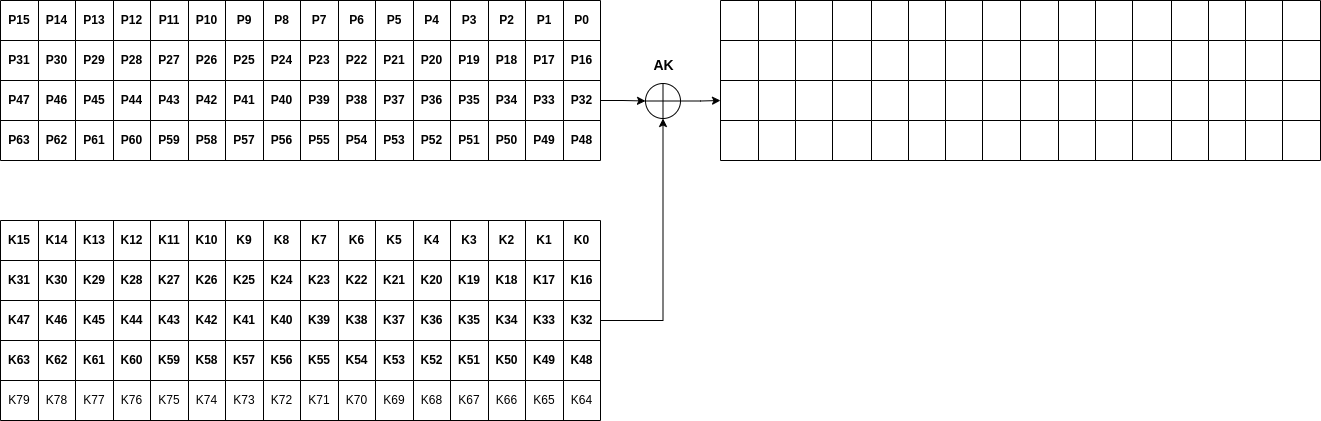
\includegraphics[width=\textwidth]{SKCrypto.drawio.png} 
        \label{fig:image1}
    \end{subfigure}
    \caption{Above diagram shows add round-key operation}
    \label{fig:two_images}
\end{figure}
    
\end{block}
\end{frame}

\begin{frame}{SubColumn (SC)}
\begin{block}{}
SubColumn parallels SubBytes, applying S-boxes to the 4 bits in each column of the state matrix.
\begin{itemize}
    \item Input to the S-box: Col(j) = $a_{3,j} || a_{2,j} || a_{1,j} || a_{0,j}$ for $0 \leq j \leq 15$
    \item Output to the S-box: S(Col(j)) = $b_{3,j} || b_{2,j} || b_{1,j} || b_{0,j}$
\end{itemize}
    \begin{figure}[H]
    \centering
    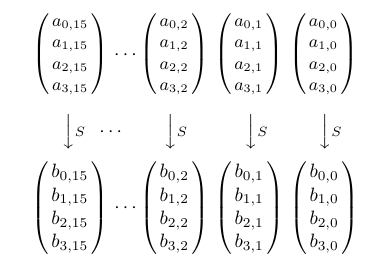
\includegraphics[width=0.4\textwidth]{SubColumn.png}
    \caption*{Figure: Above diagram shows SubColumn operation}
\end{figure}
S-box of Rectangle Cipher-
\begin{figure}
\centering
    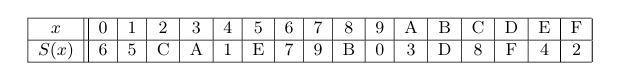
\includegraphics[width=0.8\textwidth]{S-Box.png}
    \caption*{ \textbf{Rectangle Cipher S-Box}}
\end{figure}
    
\end{block}
\end{frame}

\begin{frame}{ShiftRow (SR)}
\begin{block}{}
    It is left rotations on the rows of a state matrix,
with varying offsets for each row.
\begin{figure}[h!]
    \centering
    % First Image
    \begin{subfigure}[b]{1.0\textwidth}
        \centering
        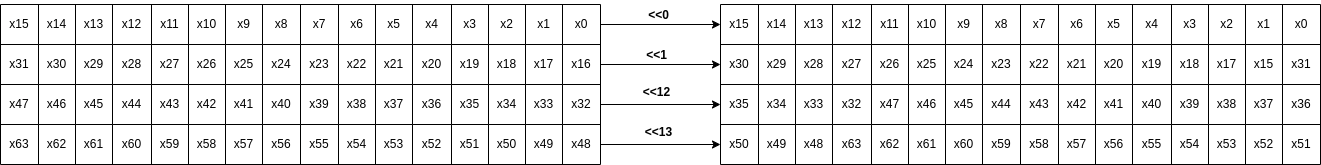
\includegraphics[width=\textwidth]{SR.drawio.png} 
        \label{fig:image1}
    \end{subfigure}
    \caption{Above diagram shows shift row operation}
    \label{fig:two_images}
\end{figure}
    
\end{block}
\end{frame}

\begin{frame}{Pseudo Code}
    \begin{block}{}
    \textbf{GenerateRoundKeys(state)}:\\
\hspace*{1cm}\textbf{for i = 0 to 24 do:}\\
\hspace*{2cm}\textbf{ARK(state,$K_i$)}\\
\hspace*{2cm}\textbf{SC(state)}\\
\hspace*{2cm}\textbf{SR(state)}\\
\hspace*{1cm}\textbf{ARK(state,$K_{25}$)}\\
    \end{block}
\end{frame}

\begin{frame}{Differential Distribution Table (DDT)}
\begin{block}{}
    \begin{figure}[H]
    \centering
    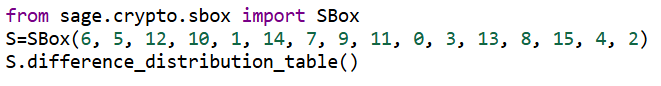
\includegraphics[width=0.7\textwidth]{Screenshot 2024-11-30 141729.png}
    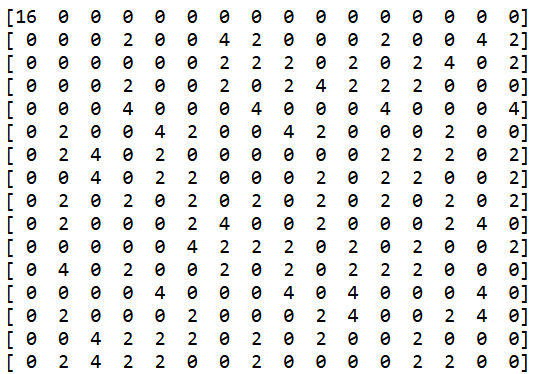
\includegraphics[width=0.7\textwidth]{Screenshot 2024-11-30 141742.png}
\end{figure}
    
\end{block}
\end{frame}

\begin{frame}{Linear Approximation Table (LAT)}
\begin{block}{}
    \begin{figure}[H]
    \centering
    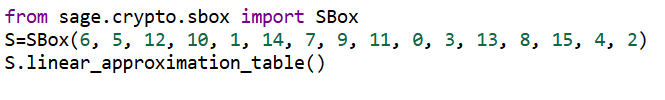
\includegraphics[width=0.7\textwidth]{Screenshot 2024-11-30 142114.png}
    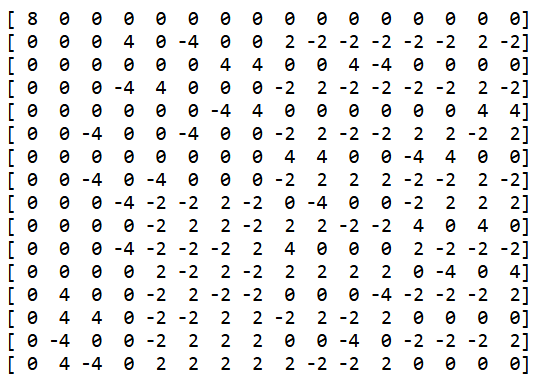
\includegraphics[width=0.7\textwidth]{Screenshot 2024-11-30 142130.png}
\end{figure}
    
\end{block}
\end{frame}

\begin{frame}{Key Schedule}
    \begin{block}{For 80-bit key}
    \begin{enumerate}
        \item SC to the bits at the 4 uppermost rows and the 4 rightmost
columns
\item Using a 1-round generalized Feistel transformation\\
$Row’_0$ := ($Row_0$ << 8) $\oplus$ $Row_1$\\
$Row’_1$ := $Row_2$\\
$Row’_2$ :=$Row_3$\\
$Row’_3$ := ($Row_3$ << 12) $\oplus$ $Row_4$\\
$Row’_4$ := $Row_0$
\item A 5-bit round constant RC[i] is XORed with the 5-bit key
state for i $\in$ (1,2,..,24).
    \end{enumerate}
        
    \end{block}
    
\end{frame}
\begin{frame}{Key Schedule}
    \begin{block}{For  128-bit key}
    \begin{enumerate}
    \item SC to the bits at the 8 rightmost columns.
    \item Using a 1-round generalized Feistel transformation\\
    $Row’_0$ := ($Row_0$ << 8) $\oplus$ $Row_1$\\
    $Row’_1$ := $Row_2$\\
    $Row’_2$ := ($Row_2$ << 16) $\oplus$ $Row_3$ 
    $Row’_3$ := $Row_0$
    \item A 5-bit round constant is XORed with the 5-bit key state
    \end{enumerate}
    \end{block}
\end{frame}

\section{Cryptanalysis}

\begin{frame}{Differential Attack}
\begin{block}{}
    \begin{itemize}
        \item Differential Cryptanalysis is one of the strongest techniques for the cryptanalysis of block ciphers.
        \item Using the algorithm based on the branch and bound method, the best differential trails from round-1 to round-15 were found.
        \begin{block}{}
            \tiny
            \centering
            \begin{array}{||c|c||c|c||c|c||}
                \hline \sharp R & \text { Prob. } & \sharp \mathrm{R} & \text { Prob. } & \sharp \mathrm{R} & \text { Prob. } \\
                \hline 1 & 2^{-2} & 6 & 2^{-18} & 11 & 2^{-46} \\
                \hline 2 & 2^{-4} & 7 & 2^{-25} & 12 & 2^{-51} \\
                \hline 3 & 2^{-7} & 8 & 2^{-31} & 13 & 2^{-56} \\
                \hline 4 & 2^{-10} & 9 & 2^{-36} & 14 & 2^{-61} \\
                \hline 5 & 2^{-14} & 10 & 2^{-41} & 15 & 2^{-66} \\
                \hline
            \end{array}
        \end{block}
        \item Using the 14-round differential propagation, we can mount an attack on the 18-round Rectangle cipher.
        \item A 25-round Rectangle cipher is sufficient to withstand this differential cryptanalysis attack.
    \end{itemize}
        
\end{block}
\end{frame}

\begin{frame}{Integral Attack}
\begin{block}{}
    \begin{itemize}
        \item Implemented Square Attack, which uses a 4-round integral distinguisher.
        \item After 4 rounds, the XOR sum in any 4-bit positions equals 0, i.e., the balanced property:
        \[
        \oplus S_{(0,0)} = \oplus S_{(1,1)} = \oplus S_{(2,13)} = \oplus S_{(3,13)} = 0
        \]
        \item Visual Representation:
        \begin{figure}[h!]
            \centering
            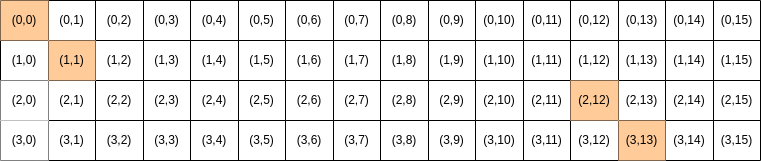
\includegraphics[width=0.6\textwidth]{diff1.drawio.png} % Replace with your image filename
            \label{fig:integral_attack}
        \end{figure}
        \item Decryption: We choose 248 plaintexts such that:
        \begin{itemize}
            \item Columns 0, 13, 14, 15 maintain the CONSTANT property.
            \item Other 12 columns maintain the **ALL** property.
        \end{itemize}
        \item $2^{48}$ Intermediate values $\implies 2^{47}$ subsets $\implies 2$ values.
    \end{itemize}
        
\end{block}
\end{frame}


\section{Software Implementation}

\begin{frame}{Software Implementation}
    \begin{block}{encryptor.py}
        \begin{itemize}
            \item Uses a 25-round encryption process with operations: AddRoundKey, SubColumn, and ShiftRows.
            \item Accepts a 16-character hexadecimal input, padding it if needed.
            \item Generates a 20-character random key for encryption.
        \end{itemize}
    \end{block}

    \begin{block}{decryptor.py}
        \begin{itemize}
            \item Reverses encryption steps using precomputed round keys.
            \item Computes all 25 round keys beforehand for accurate decryption.
            \item Outputs the decrypted plaintext as a hexadecimal string.
        \end{itemize}
    \end{block}
\end{frame}


\section{Application}

\begin{frame}{Application}
\begin{block}{}
    Encrypt message in QR codes using RECTANGLE
    \begin{itemize}
        \item encryptor.py - contains the encryption of RECTANGLE cipher 
        \item decryptor.py - contains the decryption of RECTANGLE cipher
        \item generate\_qr.py - encrypts the message and embeds it in QR code
        \item decrypt\_qr.py - scans and retrieves the plaintext from the QR-code
    \end{itemize}
        
\end{block}
\end{frame}

\begin{frame}{Generated QR Code}
\begin{block}{}
    \begin{figure}[h!]
    \centering
    % First Image
    \begin{subfigure}[b]{0.45\textwidth}
        \centering
        
\includegraphics[width=\textwidth]{message.png} % Replace 'image1.png' with your image filename
        \label{fig:image1}
    \end{subfigure}
    \hfill
    % Second Image
    \begin{subfigure}[b]{0.45\textwidth}
        \centering
        
\includegraphics[width=\textwidth]{birth.png} % Replace 'image2.png' with your image filename
        \label{fig:image2}
    \end{subfigure}

    \caption{Above QR Codes contain encrypted messages}
    \label{fig:two_images}
\end{figure}
        
\end{block}
\end{frame}
\section{Brownie Point Nominations}

\begin{frame}{Brownie Point Nominations}
\begin{block}{}
\begin{itemize}
    \item Rectangle is based on SP-Network.
    \item It is slightly similar to AES.
    \item Out of 25, the maximum of 18-rounds can be attacked.
    \item The remaining 7-rounds are for security purposes.
    \item It attains a very fast software as well as hardware performance.
\end{itemize}
    
\end{block}
\end{frame}


\section{Conclusion}

\begin{frame}{Conclusion}
\begin{block}{}
\begin{itemize}
    \item It is lightweight bit-slice block cipher.
    \item It provides applications enough flexibility.
    \item It has the ability to trigger various new cryptographic problems.
    \item Its security is encouraged.
\end{itemize}
    
\end{block}
\end{frame}



\begin{frame}{Thanks}
\begin{block}{Team Members}
	\begin{itemize}
		\item Siddhi Agarwal (12141570)
		\item Kriti Gupta (12140940)
	\end{itemize}
\end{block}
\begin{block}{Implementation Info}
	\begin{itemize}
		\item Github Link: \href{https://github.com/agaSiddhi/RECTANGLE-cipher}{https://github.com/agaSiddhi/RECTANGLE-cipher}
	\end{itemize}
\end{block}
\end{frame}

\end{document}